\documentclass[10pt,a4paper]{article}
\usepackage[utf8]{inputenc}

\usepackage[landscape,margin=1cm]{geometry}
\usepackage[ngerman,english]{babel}


% colour themes to come. KnitR?

%-------------------------

\title{\color{w3schools}NLP {\color{alert} with CLTK} \faFileTextO~ \\ {\color{black} Pre-Workshop-Workshop}}
\author{Sarah Lang}
\date{Nov. 2019}
\usepackage[default]{raleway}
\usepackage{fontawesome}
\usepackage[T1]{fontenc}

\usepackage{hyperref}
\usepackage{enumitem}
\usepackage{lipsum}

\usepackage{xcolor}
\definecolor{customcolor}{HTML}{616AC5}
\definecolor{alert}{HTML}{CD5C5C}
\definecolor{w3schools}{HTML}{4CAF50}
\definecolor{subbox}{gray}{0.60}
\definecolor{codecolor}{HTML}{FFC300}
\colorlet{xx}{customcolor}


%--------------------------Editor mode.

\usepackage
[citestyle=authoryear,
sorting=nty,	  		%Sorts bibliography by year, name, title
autocite=footnote, 		%Autocite command generates footnotes
autolang=hyphen, 		
mincrossrefs=1, 	
backend=biber]
{biblatex}

\DeclareFieldFormat{postnote}{#1}
\DeclareFieldFormat{multipostnote}{#1}
\DeclareAutoCiteCommand{footnote}[f]{\footcite}{\footcites}

\bibliography{literature}
%----------------------------------------
%--------------------------------------------------------------------------------
\usepackage{tcolorbox}

\tcbuselibrary{most,listingsutf8,minted}

\tcbset{tcbox width=auto,left=1mm,top=1mm,bottom=1mm,
right=1mm,boxsep=1mm,middle=1pt}

\newenvironment{mycolorbox}[2]{%
\begin{tcolorbox}[grow to left by=-1em,grow to right by=-1em,capture=minipage,fonttitle=\large\bfseries, enhanced jigsaw,boxsep=1mm,colback=#1!30!white,on line,tcbox width=auto, toptitle=0mm,colframe=#1,opacityback=0.7,nobeforeafter,title=#2]%
}{\end{tcolorbox}\\[0.2em]}

\newenvironment{subbox}[2]{%
\begin{tcolorbox}[capture=minipage,fonttitle=\normalsize\bfseries, enhanced jigsaw,boxsep=1mm,colback=#1!30!white,on line,tcbox width=auto,left=0.3em,top=1mm, toptitle=0mm,colframe=#1,opacityback=0.7,nobeforeafter,title=#2]\footnotesize %
}{\normalsize\end{tcolorbox}\vspace{0.1em}}

\newenvironment{multibox}[1]{%
\begin{tcbraster}[raster columns=#1,raster equal height,nobeforeafter,raster column skip=1em,raster left skip=1em,raster right skip=1em]}{\end{tcbraster}}

\newenvironment{textbox}[1]{\begin{mycolorbox}{customcolor}{#1}}{\end{mycolorbox}}

%-------------------------------
\newtcblisting{codebox}[2]{colback=codecolor!5,colframe=codecolor!80!black,listing only, 
minted options={numbers=left,style=tcblatex,fontsize=\tiny,breaklines,autogobble,linenos,numbersep=3mm},
left=5mm,enhanced,
title=#2, fonttitle=\bfseries,
listing engine=minted,minted language=#1}

%--------------------------------------------------------------------------------
\newcommand{\punkti}{~\lbrack\dots\rbrack~}

\renewenvironment{quote}
               {\list{\faQuoteLeft\phantom{ }}{\rightmargin\leftmargin}%
                \item\relax\scriptsize\ignorespaces}
               {\unskip\unskip\phantom{xx}\faQuoteRight\endlist}
               

%--------------------------------------------------------------------------------
\newcommand{\bgupper}[3]{\colorbox{#1}{\color{#2}\huge\bfseries\MakeUppercase{#3}}}
\newcommand{\bg}[3]{\colorbox{#1}{\bfseries\color{#2}#3}}

\newcommand{\mycommand}[2]{{\ttfamily\detokenize{#1}}~\dotfill{}~{\scriptsize #2}\\}
\newcommand{\sep}{{\scriptsize~\faCircle{ }~}}


\newcommand{\bggreen}[1]{\medskip\bgupper{w3schools}{black}{#1}\\[0.5em]}
\newcommand{\green}[1]{\smallskip\bg{w3schools}{white}{#1}\\}
\newcommand{\red}[1]{\smallskip\bg{alert}{white}{#1}\\}

\usepackage{multicol}
\setlength{\columnsep}{30pt}

\setlength{\parindent}{0pt}
\pagestyle{empty}

\usepackage{csquotes}

\newcommand{\loremipsum}{Lorem ipsum dolor sit amet.}






%--------------------------------------------------------------------------------
\begin{document}
\small
\begin{multicols}{3}

\maketitle
\thispagestyle{empty}
\scriptsize
\tableofcontents


\section{Natural Language Processing (NLP)}


\begin{textbox}{Terms and sub-fields}

Quantitative methods in literary studies began in the sub-field of Stylometry: 
L.A. Sherman \emph{Analytics of Literature} (1893).  Now, there are many sub-fields and different names for quantitative methods for texts and language processing\footcite[\scriptsize A fascinating introductory read on the `statistical language model', underlying computerized language processing, is][\scriptsize Don't be put off by the emphasis on mathematics, it's really a series of easy-to-understand blog posts about langauge processing.]{beautyOfMathematics} in/for the Humanities:

\red{Quantitative Text Analysis (QTA)} \green{Computational Literary Studies (CLS)}

\red{Computational Linguistics} 

\green{Text Mining}
\red{Franco Moretti's \emph{Distant Reading}}
\red{Matthew Jocker's \emph{Macroanalysis}}

\end{textbox}

\begin{textbox}{Functions of QTA}
\begin{enumerate}
    \item \red{exploratory} Exploring a corpus for potentially interesting patterns. Be pointed to interesting phenomena; find new research questions; explore the `potentials' of the text/corpus.
    \item \red{descriptive} Describing phenomena quantitatively which we already `feel' are there but we want to grasp them more `objectively'. Confirm `qualitative hypotheses quantitatively.
    \item $\to$ both are not `results'! They still require interpretation to be valid for Humanities purposes.
\end{enumerate}

\end{textbox}





\section{Intro to NLP concepts}

\begin{textbox}{Basic concepts I}
\red{Bag-of-words (BOW)}
\green{\emph{type} vs. \emph{token}}
\emph{To be or not to be.} = 6 \emph{tokens}, 4 \emph{types}.
$\to$ aus den \emph{types} wird der \emph{bag of words} aufgebaut, darin werden dann alle Vorkommnisse (\emph{tokens}) gezählt.

\red{\emph{type}} beschreibendes Kriterium

\red{\emph{token}} Analyseeinheit

\green{\emph{case-folding}} alles in \emph{lowercase} analysieren: hat vor und Nachteile (z.B. Eigennamen), am Satzanfang evtl. sinnvoll, außer für Stilometrie. Stattdessen evtl.
\green{\emph{truecaseing}}

Je nach Entscheidung bzgl. \emph{case-folding/truecasing} ist ein Wort in Großschreibung ein anderer \emph{type} als in Kleinschreibung!
\end{textbox}

\begin{textbox}{Bag-of-words}

\underline{Was geht dabei alles verloren?}
\begin{itemize}
    \item Wortstellung
    \item Zusammenhang
    \item Phrasen
    \item Reihenfolge
    \item Ironie, Sarkasmus, Negation
\end{itemize}
\end{textbox}

\begin{textbox}{Basic concepts II}

\green{Zipf'sche Verteilung (\emph{Zipf's Law})} starker (proportionaler) Abfall der Häufigkeit (und absoluten Streuung) mit zunehmendem Rang 
\begin{quote}
Zipf's law states that given a large sample of words used, the frequency of any word is inversely proportional to its rank in the frequency table. (\href{https://simple.wikipedia.org/wiki/Zipf%27s_law}{Wikipedia})
\end{quote}

\red{Stopwords} überproportional häufige Wörter (und, \emph{the}, etc.). In Listen gesammelt, meist aus der Analyse entfernt, da sie die interessanten Partien `verdecken'.
\emph{To be or not to be} = alles Stopwords.

\red{Wortfrequenzanalysen} siehe `Statistische Grundlagen'
\end{textbox}

\begin{textbox}{Unigramme Bigramme n-Gramme}

\red{Unigramme vs. n-Gramme}
\textbf{Unigram}: Jeglicher Kontext geht verloren. \\
\textbf{n-Gramme}: 
\green{\emph{sparse data}-Problem} d.h. wir haben fast nie genug Daten dafür, außer bei \emph{sehr} großen Korpora. Die Häufigkeiten werden dabei schnell so `selten', dass nichts statistisch Relevantes mehr dabei ist. Mehr als 3-5-Gramme sind daher nicht üblich. (zumal für historische Sprachen ohnehin viel zu kleine Korpora erhalten sind!)

\end{textbox}


\begin{textbox}{Basic Concepts III}
\green{KWIC (=Keyword in Context)} 
\green{Kollokation}
\green{Konkordanz}

\begin{quote}\tiny
    Unter Konkordanz (zurückgehend auf lat. \emph{concordare} „übereinstimmen“), versteht man in den Textwissenschaften traditionellerweise eine alphabetisch geordnete Liste der wichtigsten Wörter und Phrasen, die in einem schriftlichen Werk verwendet werden. Der Begriff stammt aus der Bibelwissenschaft. \punkti

    Konkordanzen sind heute in der Regel elektronisch erstellte Trefferlisten, die sich aus der Suche meist nach einem Wort oder einer Phrase, eigentlich aber aus der Suche nach jeder beliebig definierbaren Zeichenkette ergeben. In einer Konkordanz ist meistens auch die nächste sprachliche Umgebung des gesuchten Ausdrucks, der sogenannte \emph{Kontext} angeführt, also beispielsweise der gesamte Satz, in dem ein gesuchtes Wort auftritt.
    
    Als Synonyme für Konkordanz gelten fallweise die Ausdrücke \emph{Register} und \emph{Index} oder \emph{Index verborum} (‚Verzeichnis der Wörter‘). 
    
    In der Korpus- und in der Computerlinguistik haben sich zudem, auch im Deutschen, der Ausdruck \emph{Key Word in Context} sowie dessen Abkürzung \emph{KWIC} als Benennungen für den in einer Konkordanz angezeigten Suchbegriff eingebürgert.  (\href{https://de.wikipedia.org/wiki/Konkordanz_(Textwissenschaft)}{Wikipedia})
\end{quote}

\end{textbox}

\begin{textbox}{Sentiment Analysis}
\red{\emph{Sentiment Analysis}}
Eine weitere bekannt gewordene `Wörterbuch-Methode'. Man macht quasi ganz normal die Auszählung und verbindet dann die Tabelle per \emph{join} mit einem \emph{sentiment dictionary}, das Wörter in Kategorien bewertet. Allerdings passieren natürlich Missverständnisse: Bsp: Jane Austens häufigstes Nicht-Stopwort ist `Miss', aber in \emph{lowercase} (da \emph{case-folding}) wird es natürlich fehltinterpretiert als `vermissen' und damit als negatives Gefühl gewertet!
\end{textbox}



\section{Statistische Grundlagen und Theorien}
\begin{textbox}{Statistische Grundlagen}
siehe Kap. 20 DH-Einführungsbuch: Quantitative Analyse\footcite[vgl.][]{DHIntroQA}

\red{Merkmalserhebung} z.B. Worthäufigkeiten, Anzahl Orts- und Personennamen, etc. $\to$ in Tabelle festgehalten, wo jede Spalte ein Merkmal darstellt. $\to$

\green{Merkmals-Matrix} Strukturierung, in Tabellenform für Computeranalysen leicht zugänglich, aber auch Informationsverlust durch Zerstückelung.
% frequency distribution

\green{Absolute und relative Häufigkeit / Frequenzanalyse}
Absolute Häufigkeiten bringen nichts im Vergleich zu anderen Werken, die ja nicht gleich lang sind. $\to$ Feststellung der relativen Häufigkeit eines Wortes per 1000 Wörter. 

\green{Median / Mittelwert}
Damit man werkintern mit der relativen Häufigkeit etwas anfangen kann, könnte man sie mit dem Median dieses \emph{types} im Gesamtkorpus vergleichen.
Diese nennen sich dann \emph{Maße der zentralen Tendenz}, weil sie die Verteilung mehrerer Werte in einem Wert zusammenfassen. 

\green{Streuungsmaße}
Nur weil ein Werk so und so relativ häufig ist, sagt das ja nichts darüber aus, ob das Wort einfach ganz oft an einer Stelle vorkommt oder durchgehend viel verwendet wird. $\to$ Schwankungen messen. 

\green{Standardabweichung}
Pro \emph{type} beschreibt sie die Streuung: ``Wurzel aus Mittelwert der quadrierten Abweichungen jedes Einzelwertes vom Mittelwert aller Werte''.

\green{Mittelwert-Normalisierung} 
\emph{Zipf's Law}: starker Abfall der Häufigkeit (und absoluten Streuung) mit zunehmendem Rang $\to$ Vergleichbarkeit zwischen Wörtern erschwert. $\to$ Abziehen des \emph{type}-Mittelwerts (der Sammlung) von jeder Häufigkeit im Einzeltext.

\green{z-scores transformieren} um Streuung vergleichbar zu machen: Mittelwert ist dann immer 0, Standardabweichung 1. $\to$ Hinweis auf das Verhalten des \emph{types} in der Sammlung $\to$ Merkmalsskalierung.

% nochmal genauer anschauen, Zusf bisher bis Kontrastmaße

\red{Statistische Signifikanz}
Statistisch \emph{signifikant} ist schnell mal etwas. Nicht jedes signifikante Outcome ist auch \emph{relevant}. Und sagt das überhaupt etwas aus? Nein, ohne Interpretation nicht! 
\begin{quote}
     Wann haben wir ein relevantes Resultat?
     Wir müssen vorher definieren, was «Relevanz» bedeutet.
     Was ein relevanter Unterschied ist, hängt ab vom Fachgebiet/Fachwissen.
     Die Statistik hat hier keine Antwort! (\href{https://metaphor.ethz.ch/x/2017/hs/401-0603-00L/zusatzmaterial/Wo11b_Relevanz.pdf}{Quelle})
\end{quote}

\end{textbox}

\begin{textbox}{Konzepte bzw. Theorien der QTA}
\begin{quote}
    Reading `more' seems hardly to be the solution. Especially because we've just started rediscovering what Margaret Cohen calls the `great unread'. \lbrack{} Apart from ``its canonical fraction, which is not even 1 per cent of published literature''\rbrack{} there are \lbrack{}thousands of books\rbrack{} -- no one really knows, no one has read them, no one ever will.\footcite[45]{distantreading} 
\end{quote}

\red{Franco Morettis \emph{Distant Reading}} 
Vorstellung serielles Lesen vs. menschliches \emph{Close Reading}. 
Behauptet, Literaturwissenschaft wäre nicht mehr vollständig ohne quantitative Aspekte. Das serielle Lesen aber auch irgendwie `als Alternative' anstatt \emph{close reading}.

\begin{quote}
    \punkti you \emph{reduce} a text to a few elements, and \emph{abstract} them from the narrative flow, and construct a new, \emph{artificial} object. \punkti And with a little luck, these maps will \punkti possess `emerging' qualities, which were not visible at the lower level. \punkti Not that the map itself is an explanation, of course. It offers a model \punkti\footcite[53]{graphsmoretti} 
\end{quote}


\bigskip

\green{Matthew Jockers's \emph{Macroanalysis}}
Vorstellung einer Zoom-Bewegung: Die quantitative Analyse bietet Anstöße für das \emph{Close Reading}, etc.
Er fordert die Unterscheidung zwischen \emph{reading} und \emph{analysis} -- der Überblick `aus der Ferne' ist für ihn nicht `Lesen', wie etwa Morettis Benennung suggerieren würde.
\begin{enumerate}
    \item Kontextualisierung durch das \emph{zooming out}
    \item andererseits aber auch extremes \emph{close reading}: So viel Details wie dem Computer können einem Menschen fast gar nicht auffallen, weil wir Details ja gar nicht so richtig wahrnehmen.
    \item besser informiertes Verstehen der Primärtexte: die \emph{macroscale} gibt weniger `anekdotische' Beweise als das sehr genaue Lesen nur eines einzigen Texts.
    \item `harvesting findings, not facts'
\end{enumerate}

`Mixed Methods'-Ansatz, Wechselspiel

\begin{quote}
    This is not close reading; this is macroanalysis, and the strength of the approach is that it allows for both zooming in and zooming out.\footcite[23]{macroanalysis}
\end{quote}

\red{Pipers \emph{cultural analytics}}

\end{textbox}


\section{NLP-Pipeline und Korpusaufbau}
\begin{textbox}{NLP-Pipeline}
\red{(\emph{Pre-Processing})}
%$\to$ fällt in unserem Fall normalerweise unter das sog. (\emph{Pre-Processing})

\red{Tokenizer}
\textbf{Einfachste Tokenizer:} Nur der Whitespace/Leerzeichen ist Trenner. Erweiterbar durch Hinzufügen von Punktuation oder sprachinternen Spezifika.

\textbf{Sprachgebunden}, z.B. frz. \emph{l'enfant}, lat. \emph{dixitque}, en. \emph{don't} auflösen, \dots 

Wie wird mit \textbf{\emph{compounds}} (zusammengesetzen Wörtern) umgegangen?
Fremdsprachliche \textbf{Lehnwörter}, die zusätzlich noch stehende Wendungen sind (z.B. \emph{en masse})?

Geht meist ohne Wörterbuch -- für die meisten anderen NLP-Methoden müssen Wörterbücher und Grammatiken vorliegen (! ist für einen historischen Sprachstatus absolut nicht selbstverständlich) $\to$ Computer kann nicht denken und ist z.B. mit der uneinheitlichen Orthographie von frühneuzeitlichem Deutsch völlig überfordert: Methoden davon teilweise in die völlige Impraktikabilität reduziert! 

$\to$ aber geht natürlich super für moderne lebendige Sprachen, v.a. Englisch.

\begin{quote}
    \textbf{But what is a word?} We tend to think of a word as a unit of meaning that often has an analog in the real world. \punkti A computer doesn't know what a word is and certainly has no sense of what words might refer to.
    \punkti 
    Words are usually bounded by spaces and punctuation, and a computer can be told to split a long string (text) into shorter strings (words) by looking for the demarcation characters \punkti -- a process called tokenization.\footcite[283]{textvisual}
\end{quote}
\end{textbox}


\begin{textbox}{Im Detail dazu im Praxisteil}

\red{Lemmatization} Mithilfe von \textbf{Wörterbuch/Vokabular, Grammatik und morphologischer Analyse} der Wörter die Grundform (das \emph{Lemma}, wie man es im Wörterbuch hat) zu finden, damit alle Wortformen korrekt als Formen desselben \emph{type} gezählt werden können.

\red{Stemming} Wortende bis zur Wurzel abschneiden, nicht unbedingt auf linguistisch korrekte Art und Weise.

\red{Parsing}

\red{POS tagging}

\red{\emph{Named Entity Recognition} (NER)}
\end{textbox}


\begin{textbox}{Korpusaufbau I}
DH-Einführung: Kap. 16 `Datensammlungen'\footcite{DHIntroDatensammlungen}

Datensammlung nicht mit der technischen Umsetzung (Datenbank, etc.) verwechseln! (`Base of data' $\neq$ `database')

\textbf{Ablauf:} Abgrenzung des Gegenstands, Auswahl der Datensätze, Zusammenführung, Vereinheitlichung, Erheben von Metadaten (Informationen, die die Datensätze beschreiben), (ggf.) Verfügbarmachen.

\textbf{Definition des Gegenstands} der Datensammlung in Abhängigkeit von einer Forschungsfrage. 
\textbf{Mögliche Kriterien:} zeitlich, räumlich, Epoche, Genre, AutorIn / Urheber, Umfang, technische Verfügbarkeit.

\red{Grundgesamtheit}
\textbf{Gegenstandsdefinition $\to$ Grundgesamtheit,} also Gesamtmenge aller relevanten Gegenstände kann festgestellt werden. Wie steht mein ausgewähltes Korpus zu dieser Grundgesamtheit \emph{aller} in Frage kommenden Objekte? Ist es genug, um aussagekräftige (statistisch signifikante) Schlüsse zu ziehen? Im Zweifelsfall kann man immer die Fragestellung eingrenzen.

\textbf{Vollständige (!) Datensammlung:} Wenn ich mich mal entschieden habe, muss ich auch konsequent dabei bleiben, sonst wird es nichts!

\textbf{Frage nach Verfügbarkeit:} Aber falls verfügbar Frage nach Qualität der verfügbaren Inhalte (!) bzw. Nutzungsrechte, etc.

\end{textbox}



\begin{textbox}{Korpusaufbau II: Auswahlprinzipien}

\red{Repräsentatives Sample}
Umfang kann sich z.B. durch eine repräsentative Stichprobe (\emph{sample}) begrenzen:
\begin{quote}
``Representativeness refers to the extent to which a sample includes the full range of variability in a population.'' (Biber 1993, 243)
\end{quote}
$\to$ auf Grundlage der Stichprobe gültige Aussagen über die Grundgesamtheit treffen.

Gleichbehandlung aller Werke oder Vorzug dem Kanon / weiter verbreiteten Werken? Auch die `Ausreißer' mit aufnehmen? Per Zufall oder `Gütekriterien'?

\red{Balancierte Sammlung} Alternative zum repräsentativen Sample. Gezielte Konstruktion nach wesentlichen Kriterien (abhängig von der Forschungsfrage).

Korrelationen, also statistische Abhängigkeiten, zwischen Eigenschaften der Datensätze und den ausgewählten wesentlichen Kriterien sind zu vermeiden.

\red{Opportunistische Wahl} Was ist verfügbar?

\begin{quote}
     A \emph{corpus} is a body of texts (though a corpus can have only a single text). \punkti One size does not fit all.
     \punkti A digital corpus is a bit like a bag of Lego where pieces can be built up in various configurations.\footcite[281--282]{textvisual}
\end{quote}


\end{textbox}



\begin{textbox}{Korpusaufbau III: Repräsentativität}
\red{Repräsentativität}
Was wird digitalisiert und warum? Zufall? Hat `der Kanon' Priorität? Sind Texte verlässlich und verfügbar oder aber aus rechtlichen Gründen unzugänglich? Wir können leider nicht \emph{restlos alles} digitalisieren. Sind dann digitale Massenanalysen überhaupt repräsentativ? Vgl. GoogleBooks.

\begin{quote}
    By allowing a researcher to survey a larger set of documents, text mining promises to give a picture \punkti that is ``more representative'' than an account based on a few hand-selected examples. But representative of what?
    Digital libraries \punkti do not include every book ever published. Moreover, even if we had a copy of every book, the print record itself would not reflect the demographic reality of the past, since access to print has been shaped by class, gender, and race.\footcite[300--301]{textmining}
\end{quote}
\end{textbox}

\vspace{2em}


\href{https://www.springer.com/de/book/9783476026224}{
\includegraphics[width=0.2\textwidth]{dh-einf.png}}


\newpage
%-------------------------------------------------------------------------------------------------------
\section{Tools und Visualisierung}


\begin{textbox}{Informationsvisualisierung (\emph{`DataViz' / `InfoViz'})}
Siehe Kapitel 23 `Informationsvisualisierung' (DH-Einführungsbuch)\footcite[vgl.][]{DHIntroRehbeinInfoviz}


Grafische Elemente als Kommunikationsmittel \sep
visuelle statistische Darstellungen als Repräsentationen von Sprache \sep
Entlastung des Geistes bei großes Datenmengen: \emph{snapshot} statt Gesamtwerk. \sep `method for seeing the unseen' \sep durch die Visualisierung werden abstrakte Daten räumlich angeordnet \sep oft interaktive Schnittstellen, um den Denkprozess zu begleiten 

\bigskip

\green{Funktionen}
\begin{enumerate}
\item \textbf{anschauliche Präsentation} von Daten/Ergebnissen, am Ende des Forschungsprozesses
\item \textbf{konfirmative Analyse:} Sichweisen (\emph{views}) auf Daten erzeugen, die erlauben, Hypothesen zu verifizieren oder falsifizieren. Teil des Forschungsprozesses.
\item \textbf{explorative Analyse:} nicht hypothesengetrieben, Strukturen oder Trends erkennen. $\to$ interaktive Werkzeuge, zu Beginn des Forschungsprozesses
\item \textbf{Visualisierung} (z.B. Storytelling)
\end{enumerate}

\red{makros vs. mikro} Einerseits Aufzeigen übergeordneter Strukturen (`distant reading'), aber auch Detaileinblick in die Daten.

\green{Vorgehen}
\emph{raw data} $\to$ (Vorverarbeitung) $\to$ \emph{data tables} $\to$ \emph{visual structures} $\to$ \emph{views}.

$\to$ Tufte 1983: \emph{A silly theory means a silly graphics.}
% bis S. 334: weiter mit Datentypen, visuelle Strukturen
\end{textbox}

\begin{textbox}{Nie vergessen}

\begin{quote}
        \emph{A fool with a tool is still a fool!} (\href{https://en.wikiquote.org/wiki/Talk:Grady_Booch}{Grady Booch})
    \end{quote}

\end{textbox}

\begin{textbox}{DataViz II: Links zu Tools}
\href{http://www.sthda.com/english/wiki/text-mining-and-word-cloud-fundamentals-in-r-5-simple-steps-you-should-know}{Intro to WordClouds in R} \sep \href{http://www.sthda.com/english/wiki/word-cloud-generator-in-r-one-killer-function-to-do-everything-you-need}{Detailerklärung zur WordCloud selbst, aus derselben Quelle} \sep
\href{https://cran.r-project.org/web/packages/wordcloud/wordcloud.pdf}{wordcloud-Package-Dokumentation}

\href{http://wordseer.berkeley.edu/}{WordSeer (Berkeley} (Visualisierungs- und Textanalysetool, muss installiert werden) \sep
\href{https://www.textarc.org/}{Textarc-Visualisierung} (evtl. nicht verfügbar) \sep 
\href{http://lexos.wheatoncollege.edu/}{Lexos}: Von Pre-Processing über Analysen (mehrere Texte) bis zur Visualisierung (z.B. Rolling Window). \sep
\href{http://textvis.lnu.se/}{Text Visualization Browser} \sep 
\href{https://www.overviewdocs.com/}{Overview-Tool} (Download) \sep 
\href{http://tapor.ca}{Tapor-Toolübersicht} \sep
\href{http://www.deutschestextarchiv.de/doku/DDC-suche_hilfe}{Deutsches Textarchiv Hilfe}
\end{textbox}




\begin{textbox}{DataViz III}
\green{Frage nach der Aussagekraft der Daten}
\begin{quote}\scriptsize
Nur aus der bloßen Existenz von Daten kann nicht auf deren Bedeutsamkeit geschlossen werden, und nicht alles, was (in einem bestimmten Kontext) bedeutsam ist, hinterlässt messbare Datenspuren.

Ein weiterer Schritt ist durch den Forscher selbst zu vollziehen: Visualisierungen sind häufig gut geeignet, um Strukturen und Muster zu zeigen. Sie liefern allein für sich aber keine Erklärungen. Mit anderen Worten: Korrelationen oder Koinzidenzen, wie sie sich vielleicht in den Daten erkennen lassen, bedeuten noch keine Kausalität, eine Wiederkehr noch keine Gesetzmäßigkeit. Erklärungen lassen sich erst durch Interpretation der Visualisierungen, oft unter Bezugnahme von anderen Daten, Quellen oder auch Methoden, durch den Forscher folgern. \emph{(Rehbein 2017, 341--341)}
\end{quote}
\end{textbox}


\begin{textbox}{Rolling Window}
\href{http://www.thomaswilhelm.eu/shakespeare/output/hamlet.html}{To See Or Not to See: Shakespeare-Visualisierung} \sep Annotationsbasiert

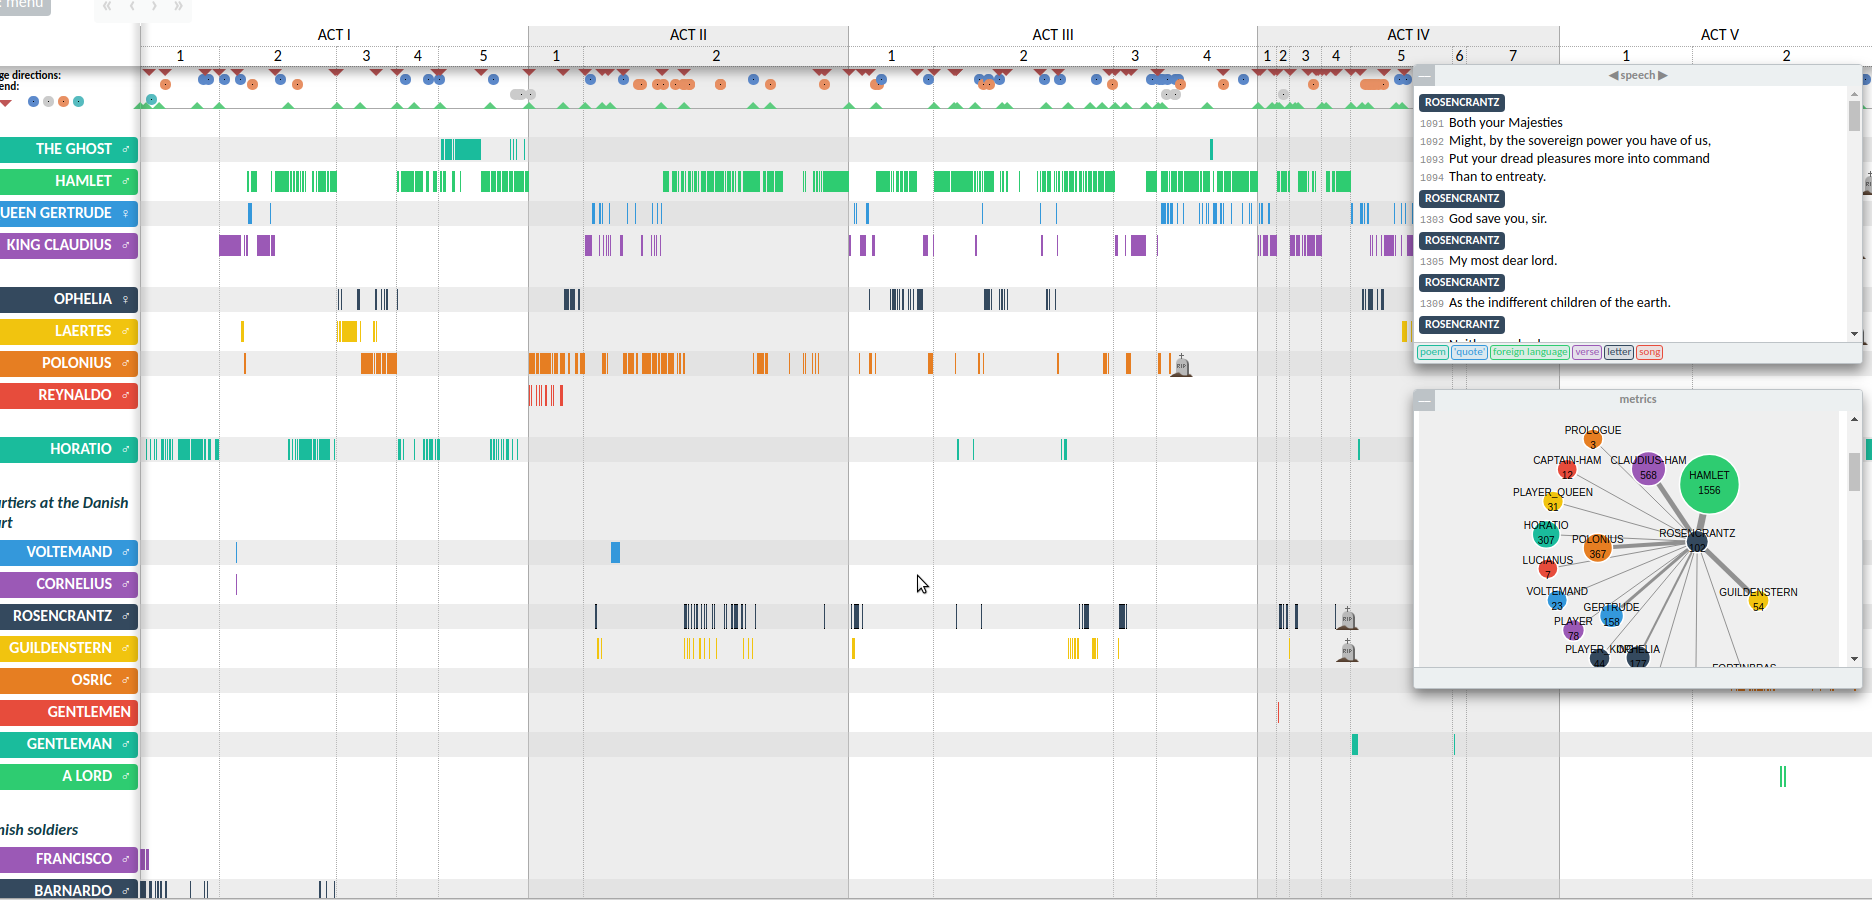
\includegraphics[width=\textwidth]{toSeeOrNotToSee.png}
\end{textbox}


\begin{textbox}{\href{https://www.jasondavies.com/wordtree/}{WordTree}}

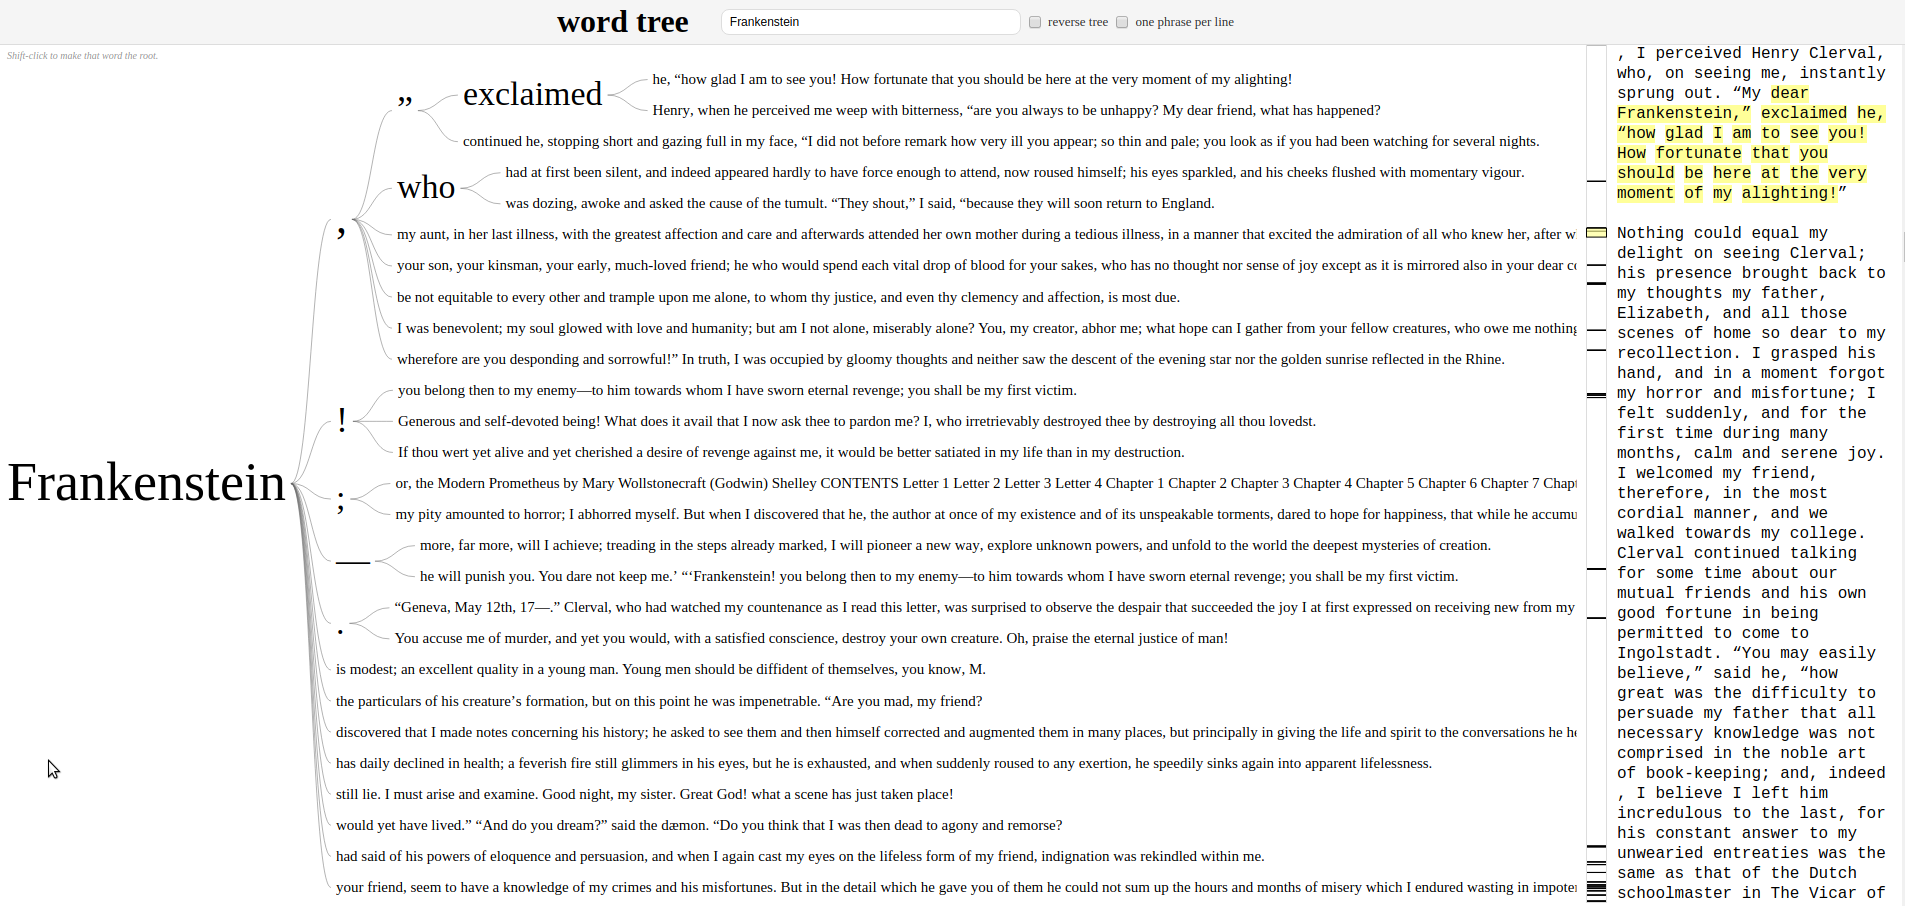
\includegraphics[width=\textwidth]{wordTree.png}
\end{textbox}

\begin{textbox}{\href{https://voyant-tools.org/}{Voyant Tools}}
\href{https://blogs.reed.edu/ed-tech/2017/03/text-analysis-using-voyant-tools/}{Blogpost zu Voyant} \sep features many standard functions for single and multiple documents \sep XML input possible as well

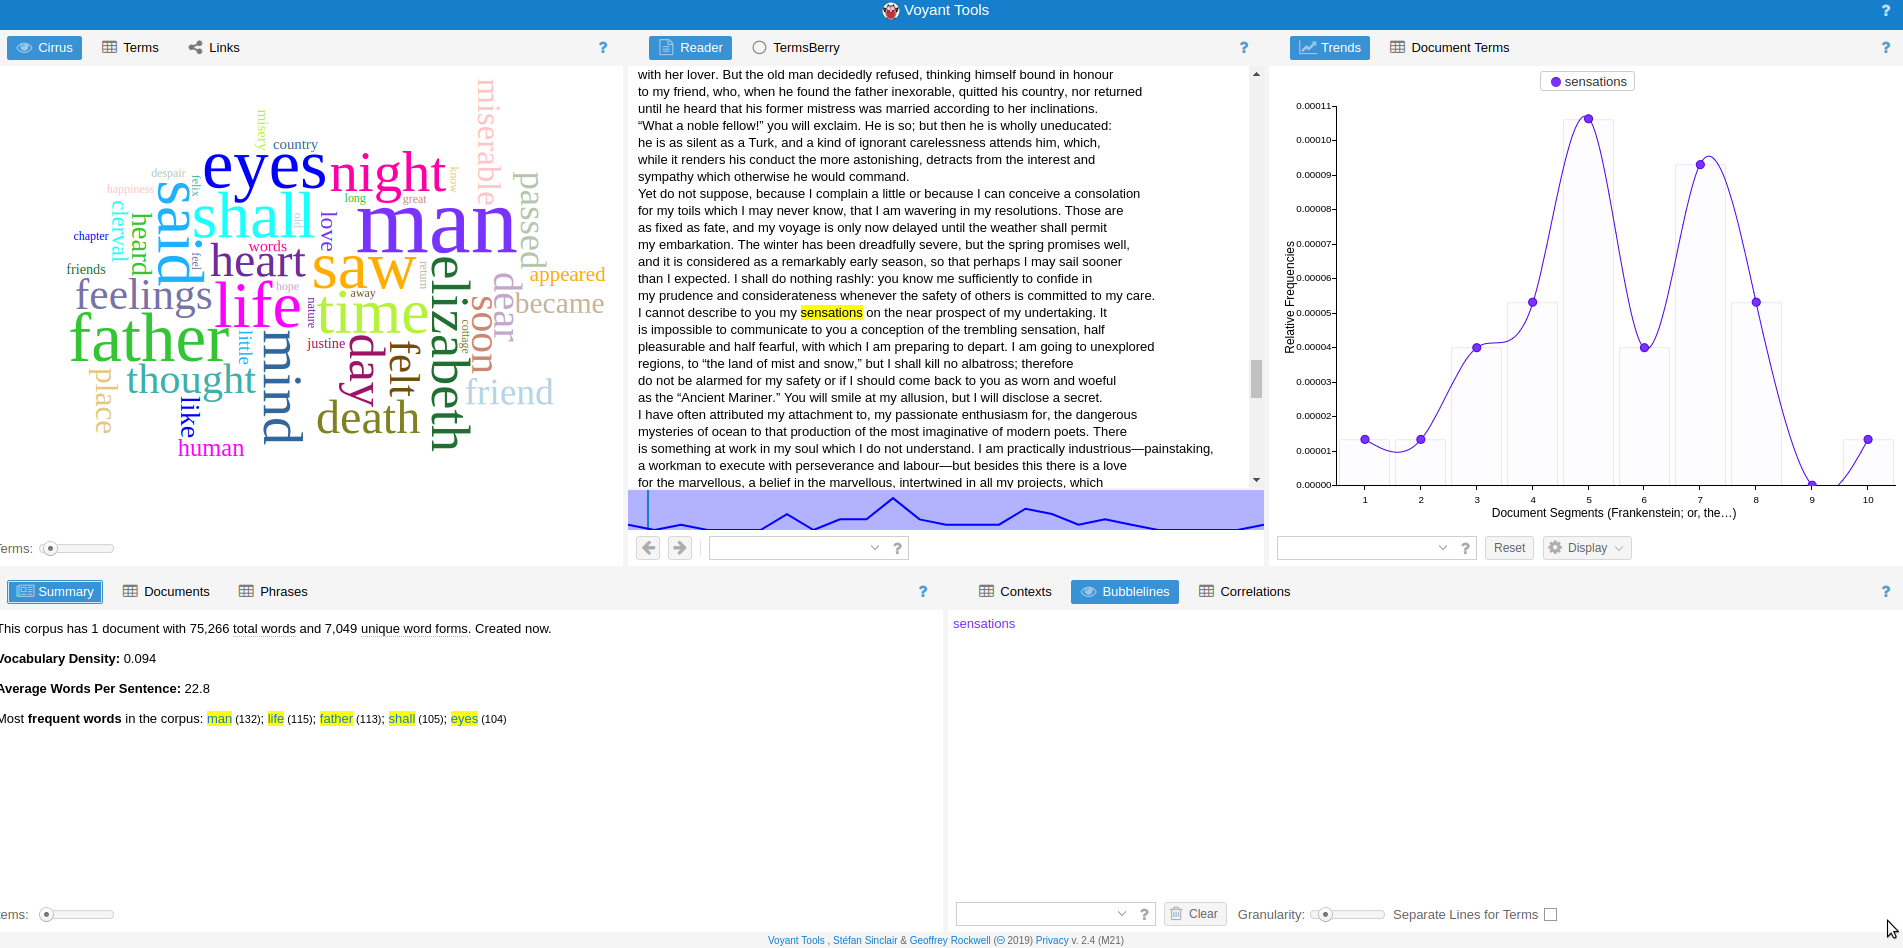
\includegraphics[width=\textwidth]{voyant.png}
\end{textbox}



\begin{textbox}{\href{https://books.google.com/ngrams}{Google Books N-Gram Viewer}}
\href{https://firstmonday.org/ojs/index.php/fm/article/view/5567/5535}{Shai Opir: Bsp. zu `Truth'}

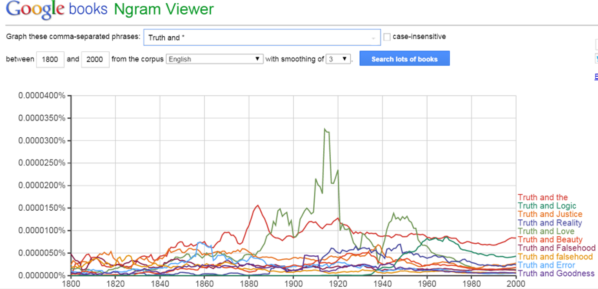
\includegraphics[width=\textwidth]{googlengramstruth.png}
\end{textbox}

\begin{textbox}{NLP-Tools}
\bg{w3schools}{white}{Stanford CoreNLP} \\
\href{https://stanfordnlp.github.io/CoreNLP/tutorials.html}{Stanford CoreNLP} \sep 
\href{https://corenlp.run/}{Online-Tool für CoreNLP} \sep 
\href{https://interviewbubble.com/getting-started-with-stanford-corenlp/}{Einsteiger-Tutorial zu CoreNLPs Funktionen}

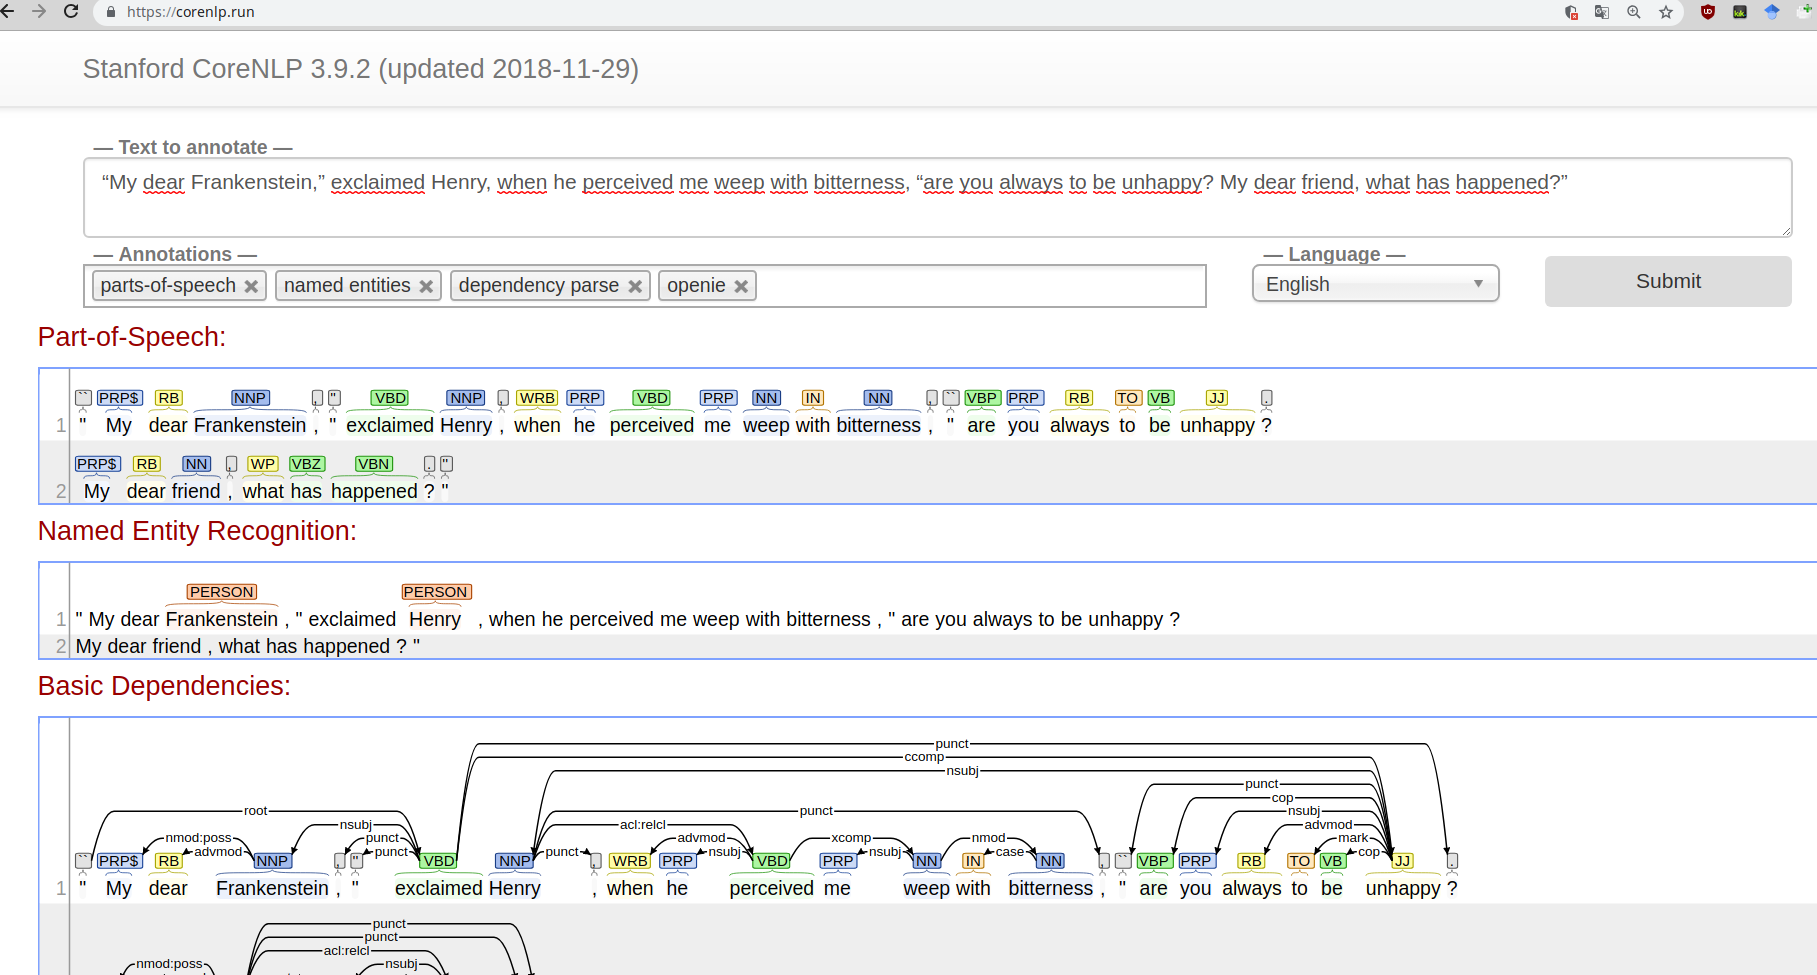
\includegraphics[width=\textwidth]{frankenstein-corenlp.png}


\href{http://www.wordandphrase.info/}{Word and Phrase}: Konkordanzen, Frequenzlisten, Texte analysieren (ein ganzer Roman scheint ihm zu viel zu sein)

\href{https://weblicht.sfs.uni-tuebingen.de/weblicht/}{Weblicht}

\end{textbox}



\begin{textbox}{\href{http://wordwanderer.org/}{WordWanderer}}
Konkordanz, Beziehungen zu anderen Wörtern, etc. Vom einen Begriff zum nächsten hangeln, \dots

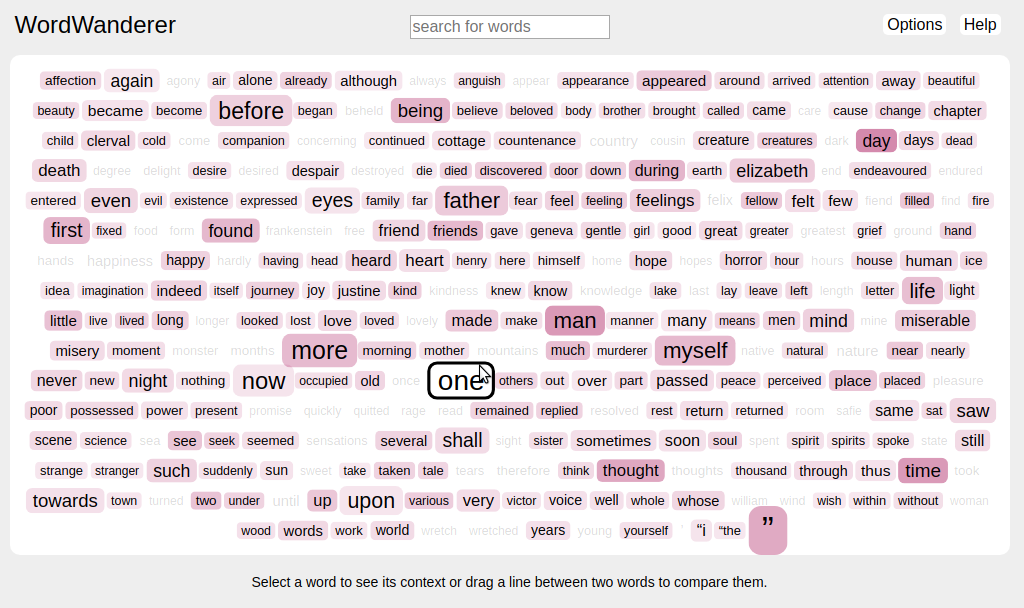
\includegraphics[width=\textwidth]{wordwanderer1.png}

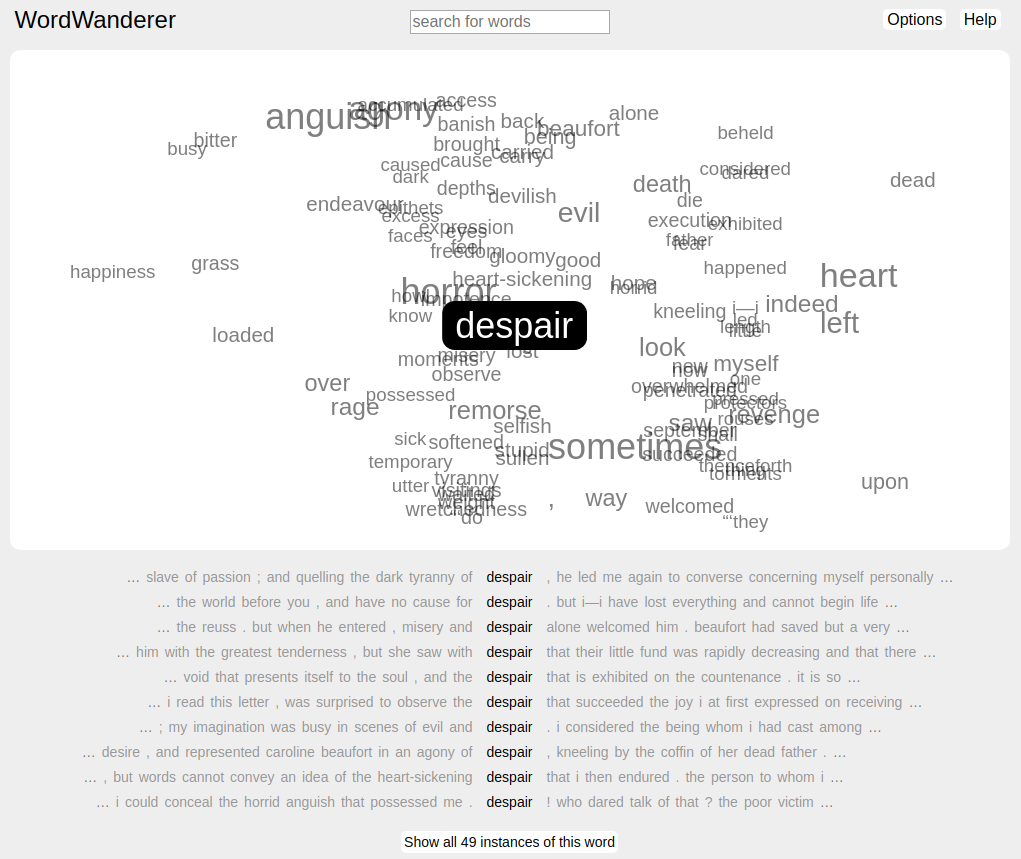
\includegraphics[width=\textwidth]{wordwanderer2.png}

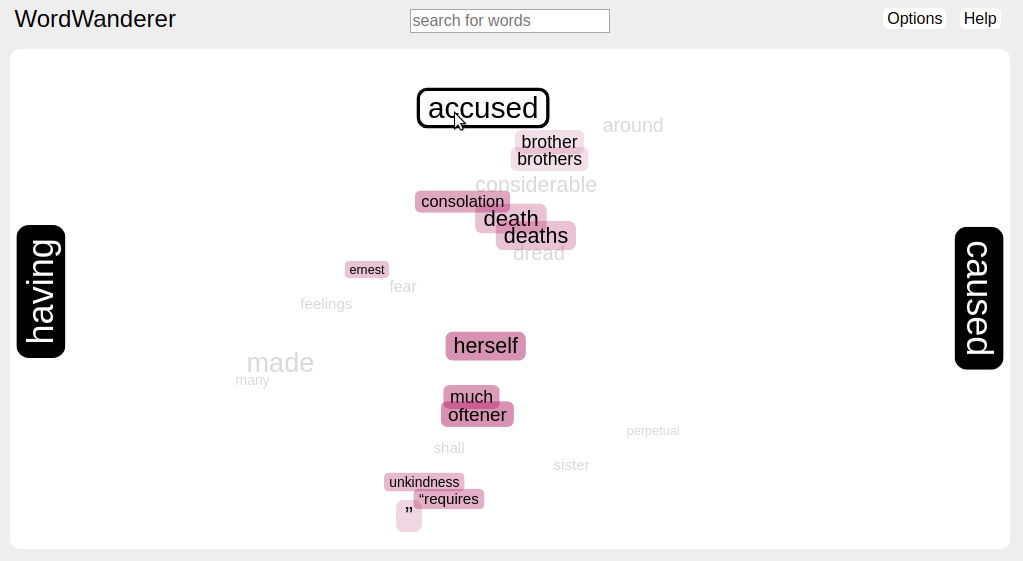
\includegraphics[width=\textwidth]{wordwanderer3.png}
\end{textbox}




\section{Grundbegriffe der Programmierung}

\begin{textbox}{Communicating with computers I}
\green{Algorithm} Recipe providing a formalized way to automate carrying out a task. Doesn't have to be noted down in a particular programming language yet, can be in `pseudo-code' (``Whenever you find a verb, do this. When you find a noun, do that.'' etc.)

\green{Algorithmic thinking} The existence of this term  hints at the fact that computers don't think like humans do, in fact, they don't think at all. A beginner needs to get to know ways of communicating effectively with a computer. This involves experience, but at a higher level also requires a certain background knowledge about the inner workings of computers (i.e. what are data types, how are libraries built, what parameters and arguments do functions expect and what do they return?)
\end{textbox}

\begin{textbox}{Communicating with computers II}
\red{Source code and compiled code}
Source code is what we see and write. However, a computer can only understand machine language (1s and 0s), so we need to `bridge this gap'. There are two ways of doing this: Either, we need to `press a button' (which might not always be a litteral button in a normal programming language, but is -- for example -- when you compile \LaTeX{} code into a PDF on Overleaf\dots) and then the code gets compiled. It produces an executable as output which can, in turn, be executed. Instead of compiled and interpreted, we can also say static and dynamic.
Or we use an `interpreted' language where this `compiling process' is done, line by line, while to code runs. Python is such an interpreted language. `Interpreting' at runtime is a bit slower and it can mean that the compiler won't be there at (the non-existant) compile time to inform you about some inconsistencies in your code. But in this case, you will have to `run' it more frequently anyway, so it probably doesn't make a difference and standard code editors will help with pointing out inconsistencies anyway. You basically get your error messages one way or the other. Which leads us to the next point\dots
\end{textbox}

\begin{textbox}{Debugging errors and error handling I}
\green{Debugging} is the act of cleaning up your code when there are errors in it which prevent it from working correctly, as intended or from running at all. The term comes from a time when computers were huge an litterally had to be debugged because bugs were stopping the wires from working correctly. There are different types of errors, most importantly:

\red{Syntax errors} mean that you didn't respect the conventions of your programming language. Like spelling and grammar mistakes in normal writing.

\red{Logic errors} are hard to detect since the conventions of the programming language are respected and automated checking tools might not find them. An example would be passing nothing to a function (indirectly and thus, invisibly) and, thus (obviously but not obviously) getting incorrect results (`Null reference error', usage of wrong conditional operator = design flaw). Usually these are `bigger' errors in the program flow compared to the more localized syntax errors (typos, missing semicolon or closing brackets, etc.).
\end{textbox}

\begin{textbox}{Debugging errors n error handling II}
\red{Semantic errors} mean that the code runs alright, but it doesn't do what you intended it to do. Remember that the computer will do exactly what you tell it to do even if this is not, in fact, the same as what you intended to do. (This happens a lot, not only to beginners).

\red{Runtime error} A program crashes due to unexpected input but the compiler can't know someone will input something which will cause the crash (such as an unexpected and thus uncaught division-by-zero error which you should actually prevent). There are many recurring types of errors which consequently have received their own names, such as index-out-of-range error or off-by-one error, to name to most well-known examples.
\end{textbox}

\begin{textbox}{Debugging errors n error handling III}
\red{Error handling} Errors should be handeled in your program flow, this means they should be anticipated, `caught' or `thrown'. An error message will specify what kind of problem happened which makes debugging easier. An expected and thus properly handeled error prevents the program from crashing whenever something problematic happens (which shouldn't happen!). If you have an advanced error handling in place, your program will know how to react when different types of errors happen. However, this is maybe overkill for tiny script-like programs where a crash is not an issue. 
\end{textbox}

\begin{textbox}{IO}
\green{Input and Output} Input and output (sometimes referred to as I/0) are base concepts of how computing works: You give input to a function or computer program and expect it to return a certain output. In between, some processing happens.

This is actually the same principle in a function you know from maths, if this helps you. For example, in image processing, every pixel of an image has a colour code stored in some data format (which you don't need to worry about). Just know that it has a numeric value which can be used as input for a function. So when processing an image in an image manipulation programme (such as turning it to grayscale), every colour value gets inputted into a function which makes some decisions, such as: If the colour value is above threshold XY, make it black - if it is below it, make it white. So in the "output graph", like a function graph in maths, you get these transformed values which can, in turn, be "put back" (written onto) their old locations in the coordinate system that is the grid behind what you see as a digital image.

The following terms will give you more detailed understanding of how exactly these functions work, but keep the image of maths functions in the back of your mind. Computer functions are not exactly the same, but the principle is similar.
\end{textbox}

\begin{textbox}{Abstraction}
\green{Variable} A variable is a container for storing information. A variable is a container for storing information, kind of like in maths where a variable is a placeholder for a yet unkown value. It is named (such as 'x' in maths). Calling the name usually causes it to give you its `contents'.

\green{Function} A function is a generalized bit of code, made for general-purpose reuse. So essentially, you abstract what is being done. Instead of ``process my document test.txt'' you would write something like \texttt{process(text)} and would be able to pass a document of any name to this \texttt{process()} function like \texttt{process("test.txt")} or \texttt{process("unicorn.txt")}. This has the awesome advantage that it doesn't matter whether your document is called `test' or `unicorn' or, in fact, any other crazy name you can come up with. A function usually has a `signature' that means a list of what parameters you pass to it (in the definition of a function, you say which type of data will be inputted) and what it will return. 
\end{textbox}

\begin{textbox}{Abstraction}
\green{Parameter} is a variable in the declaration of a function. Together with variables (and parameters \emph{are} a type of variable), parameters contribute to the abstraction of functions. This is a good thing. 

Imagine you would (and you will in the process of developping a function) write multiple lines of code. Once you got the thing working, you want to apply it to all the other things this automated processing needs to be applied to. If you don't create a function where this gets abstracted, you have to copy all those lines over and over again, only to make minor changes in the actual code. This is a situation that practically screams ``Define a function for this repetitive behaviour!'' at you. You should listen to the call. Once it's abstracted and you realize a change needs to be made, you need to make that change exactly once and not in every single line of the code you copy-and-pasted around which now clutters your editor. This means, with writing a function, we have reduced redundancy -- and in computer things, we always want to reduce redundancy. Amen. However, the variables and parameters are abstract stand-ins. Their names can act like placeholders. This can be quite confusing to a beginner. The point is that this abstract placeholder (parameter) in a function is not the same thing as the actual content you pass to the function (which is called the `argument', see below):
\end{textbox}

\begin{textbox}{Abstraction}
\green{Argument} is almost the same as a parameter, but the difference is that it means the actual value which gets passed to the function. So when using a function, you can pass the number 3 to it. In the definition/declaration, you say that an integer variable will be passed to it (=the parameter is an integer type value). 

\green{Return value} What a function will return as a result. This has a `return type', specifying which data type will be returned.  This can sometimes be good to know so that we don't get confused in further processing steps. However, the point about the whole function-abstraction-thing is that we really shouldn't need to know exactly how the processing is done in a function. We only need to know what we put int (input) and what we expect to get out of it (output). This makes it easier to build really complex programs where you don't want to have to worry about how excatly things were implemented in the detailled single processing steps.
\end{textbox}

\begin{textbox}{Reuse is Reduction of reundancy}
\green{Library} A library (or package) is essentially nothing else than a bunch of functions, only that when you load them into your program, you can profit from (usually) really well-done and maintained functions somebody else made. Using libraries, you can accomplish quite something writing very little code yourself. If not for practice purposes, it is always better to reuse a standard library rather than writing things yourself -- package maintainers are experienced experts and might have taken things into account which you didn't.
When you use code from a library, it means that this code is not part of the standard repertoire (`vocabulary') of your language: It is a set of functions made using this standard repertoire just as your own functions are. When you invoke or `load' them, it's essentially as though the computer would just copy their text into your document behind the scenes (and this is exactly what happens behind the scenes). 
By combining and reusing libraries, you can be really efficient and ``stand on the shoulders of giants'', as they say.
Functions coming from libraries can have the name of their library prefixed as a `namespace'. This can sometimes be a little confusing, especially for beginners because it obscures where which names belong to in longer expressions and requires you to know/remember from which libraries your used functions come.

\textbf{Redundancy is always an unnecessary source of error.} Except for in data archiving. Here, redundancy is security.

\end{textbox}

\begin{textbox}{Program Flow and Flow Control I}
In the beginning, we learned that an algorithm (and thus, also it's concrete \emph{implementation}, a program) is essentially a cooking recipe which allows us to automate things which are simple enough so they lend themselves to being automated. Sometimes, even things which look complicated at first can be reduced to simpler substeps. This is called the \textbf{`divide et impera' principle} in computer programming. 
\end{textbox}

\begin{textbox}{Program Flow and Flow Control II}
However, cooking recipes always expect the same input (the ingredients, so to speak). If the input differs from what's specified (even just a tiny little bit!), the computer really doesn't know what to do with it because the computer doesn't think and doesn't have common sense. These situations where a computer doesn't `get' simple things and doesn't compensate for our little inconsistencies (such as typos) can be irritating. So please remember always that the computer doesn't think. It's not its fault. \emph{You} made the mistake, so go and correct it. To make our programs more robust, we can use flow control, that is: some simple rules in the form of if-then conditions or behaviour which gets repeated as many times as needed or as long as there is still input. These regulate what we call 'program flow'. There are a few options available, see examples below.
\end{textbox}

\begin{textbox}{Program Flow and Flow Control III}
\red{Loop} means repeating an action for a specified number of times. If something goes wrong in the definition of the ending condition (which always need to be defined!), you can end up with an `infinite loop' which will cause the program to hang or `freeze' and eventually crash. For-loops repeat for a fixed amout of times, while loops repeat while a condition is true, do-while-loops execute at least one time and then behave as while-loops.

\red{Conditional} is an if-then-type decision which can be used to regulate program flow. You can define multiple if cases, but also if-else and else cases which will handle everything which doesn't match the condition.
\end{textbox}

\begin{textbox}{Data types}
Suffice it to say, for now, that there are different ways of storing data. As a beginner, especially if you're using a loosely typed language such as Python, this isn't all that important at the beginning so I don't want to be too verbose as not to confuse you with irrelevant facts.

\green{Data types} 
There are simple (`primitive') data types, such as integer, characters, floating point numbers or strings; as well as complex data types such as hashmaps, lists, dictionaries, etc. which are specific to the implementation in a programming language. There are also ways for you to define your own complex data types (such as defining that if you want to store data on people, you need their names, ages and addresses and and address always consists of X, Y and Z).
Python is a `dynamically (or weakly) typed' language, so you don't need to perform specific operations yourself (as opposed to `strongly typed' languages like C) such as:

\green{Type-casting} means to `change' data from one type to another. A classic example is that `1' if typed into a terminal, actually is a string, not a number to the computer. In order to calculate with it, you need to change it to an integer. But this is not an issue in Python, so don't worry about that now.
\end{textbox}

\begin{textbox}{Various}
\red{Script / Scripting} Scripting in a terminal is not the same thing as programming or writing software (which contains memory allocation, error handling, etc.). 

\begin{quote}\tiny
    \textbf{To get a computer to do anything, you (or someone else) have to tell it exactly -- in excruciating detail -- what to do. Such a description of ``what to do'' is called a \emph{program}}, and \emph{programming} is the activity of writing and testing such programs.
    \punkti The difference between such \lbrack{}everyday\rbrack{} descriptions and programs is one of degree of precision: \textbf{humans tend to compensate for poor instructions by using common sense, but computers don't.}
    \punkti when you look at those simple \lbrack{}everyday\rbrack{} instructions, you'll find the grammar sloppy and the \textbf{instructions incomplete.} A human easily compensates. \punkti In contrast, computers are \emph{really} dumb.\footcite[][44. Hervorhebung hinzugefügt.]{stroustrup}
    
    We also \punkti to assume ``common sense''. \textbf{Unfortunately, common sense isn't all that common among humans and is totally absent in computers} (though some really well-designed programs can imitate it in specific, well-understood cases).\footcite[35. Emphasis added.]{stroustrup}
\end{quote}
\end{textbox}

\begin{textbox}{Programming in the DH}
\begin{itemize}
\item mostly rather `scripts' than actual programs (that's called research software engineering \#RSE)
\item you really only need enough programming knowledge to be able to:
\begin{itemize}
\item read and understand other people's code
\item modify it a bit
\item basics of \emph{debugging}
\end{itemize}
\item today, programming is mostly knowing libraries and making the most of code reuse. In the early days, everybody used to write everything themselves which resulted in overall worse quality code and much time lost programming stuff somebody else had already done (and mabye worse than they had done it).
\item much can be done using packages and lightweight \emph{scripting} without really knowing how to program 
\item $\to$ passive knowledge more than active mastery
\end{itemize}
\end{textbox}

\newpage
\section{Python}

\begin{textbox}{Python}
\href{https://docs.python-guide.org/}{Hitchhiker's Guide} \sep 
\href{https://hourofpython.trinket.io/a-visual-introduction-to-python#/welcome/an-hour-of-code}{Visual Intro with Turtle} \faBug \sep  \href{https://www.w3schools.com/python/python_intro.asp}{Learn Python Tutorial}
\begin{quote}
Python is an interpreted high-level programming language for general-purpose programming. Created by Guido van Rossum and first released in 1991, Python has a design philosophy that emphasizes code readability, notably using significant whitespace. \punkti

Python features a dynamic type system and automatic memory management. It supports multiple programming paradigms, including object-oriented, imperative, functional and procedural, and has a large and comprehensive standard library. (\href{https://en.wikipedia.org/wiki/Python_(programming_language)}{Wikipedia})
\end{quote}

\bgupper{w3schools}{white}{.py}

\end{textbox}

\begin{textbox}{The Zen of Python}

\begin{quote}\scriptsize
Beautiful is better than ugly. \\
\textbf{Explicit} is better than implicit. \\
Simple is better than complex. \\
Complex is better than complicated. \\
Flat is better than nested. \\
Sparse is better than dense. \\
\textbf{Readability counts.} \\
Special cases aren't special enough to break the rules.  \\
Although practicality beats purity. \\
\textbf{Errors should never pass silently.} \\
Unless explicitly silenced. \\
\textbf{In the face of ambiguity, refuse the temptation to guess.} \\
There should be one -- and preferably only one -- obvious way to do it. \\
Although that way may not be obvious at first unless you're Dutch. \\
Now is better than never. \\
Although never is often better than *right* now.\\
If the implementation is hard to explain, it's a bad idea. \\
If the implementation is easy to explain, it may be a good idea. \\
Namespaces are one honking great idea -- let's do more of those! \\
(\href{https://en.wikipedia.org/wiki/Zen_of_Python}{Wiki} \& \href{https://docs.python-guide.org/writing/style/#zen-of-python}{Zen of Python} \& \href{https://docs.python-guide.org/writing/style/#zen-of-python}{Hitchhiker's Guide to Python})
\end{quote}
\end{textbox}

\begin{textbox}{Python data types}
Interactive tutorials: \href{https://hourofpython.com/}{Hour of Python}

\red{Lists: related things}
Python offers a tool called lists to keep track of related `things', or values.

\begin{codebox}{py}{Lists}
grades = [97, 62, 85, 76, 99, 93]
grades[0] # get by index. output: 97 (IndexError if index non-existant)
names = ['Anna', 'Bob']
container = [grades, names] # nested lists using variables
an_empty_list = []
grades.append(42)
grades.insert(2, 'spam') # [97,62,'spam',85,76,99,93,42]
# extending with + or 
grades.extend(['foo'])
del grades[0:2]
grades.pop(3)
grades.remove(85) # will remove first occurrence of value (ValueError if non-existant)
# ['spam', 76, 93, 42, 'foo']
\end{codebox}

\bg{alert}{white}{Dictionaries: key--value} built-in to Python, for storage, to translate \textbf{keys} to \textbf{values}.

\begin{codebox}{py}{Dictionaries}
foods = {'a': 'apple', 'b': 'banana', 'c': 'cookie'}
foods['d'] = 'dates'
y = {'spam': 'eggs'}
x.update(y) # merge y into x
foods['d'] # dates 
# for the getter: KeyError if search by value
del foods['d']

\end{codebox}
\end{textbox}

\begin{textbox}{Getting Started}
If working with a terminal/prompt, `\verb|>>>|' indicates the terminal is ready for you and waiting for input. In Jupyter Notebooks, get yourself the first empty cell and get going. \texttt{CTRL+ENTER} to compile. \texttt{\lbrack{}*\rbrack{}} means it's still compiling. When it's done, \texttt{*} will be replaced by a number.

\red{Start by using Python as a simple calculator}
Enter things like: \texttt{2 + 5 * 4 - 8 / 9}.
See what happens, understand how braces work. If you disrespect some of Python's conventions, don't worry, you will be notified in an error message \faSmileO 

\green{Indentation}
Many languages use brackets to indicate blocks of code which belong together. Python, in its (somewhat extreme) simplicity, has neither brackets nor semicolons.
Code blocks which belong together are marked out as such by indentation alone. Thus, you need to exercise special caution -- if you get errors, it might be for this reason. Whereas in other languages, typical syntax errors would be missing closing brackets or semicolons.
\end{textbox}

\subsection{Installing Python and Jupyter Notebooks}

\begin{textbox}{Working with Jupyter Notebooks I}

\begin{quote}
Jupyter Notebook App (formerly IPython Notebook) is an application running inside the browser. \punkti The Jupyter Notebook App can be executed on a local desktop requiring no internet access \punkti or can be installed on a remote server and accessed through the internet. (\href{https://jupyter-notebook-beginner-guide.readthedocs.io/en/latest/}{Tutorial})
\end{quote}

\begin{enumerate}
    \item Download the \href{https://www.anaconda.com/distribution/}{Anaconda Distribution}, Python \textbf{3}, 64 bits.
    \item The Jupyter Notebook App can be launched by clicking on the Jupyter Notebook icon installed by Anaconda in the start menu (Windows)
\end{enumerate}
\mycommand{jupyter notebook}{typing in a terminal (cmd on Windows)}
\mycommand{anaconda-navigator}{Starting Anaconda GUI (in Linux)}
\end{textbox}

\begin{textbox}{Working with Jupyter Notebooks II}
\begin{quote} 
    The astute reader may have noticed that the URL for the dashboard is something like \protect\url{http://localhost:8888/tree}. Localhost is not a website, but indicates that the content is being served from your local machine: your own computer.
    
    Jupyter’s Notebooks and dashboard are web apps, and Jupyter starts up a local Python server to serve these apps to your web browser, making it essentially platform independent. 
    
    \punkti Each \texttt{.ipynb} file is a text file that describes the contents of your notebook in a format called JSON. 
    
    \punkti A code cell contains code to be executed in the kernel and displays its output below.
    
A Markdown cell contains text formatted using Markdown and displays its output in-place when it is run.
The first cell in a new notebook is always a code cell. Let’s test it out with a classic hello world example. Type \texttt{print('Hello World!')} into the cell and click the run button in the toolbar above or press \texttt{Ctrl + Enter}. (\href{https://www.dataquest.io/blog/jupyter-notebook-tutorial/}{Tutorial})
\end{quote}
\end{textbox}


\begin{textbox}{Working with Jupyter Notebooks III}
Alternative for experienced Python users: 
\green{Installing Jupyter with pip}
Jupyter installation requires Python 3.3 or greater, or Python 2.7. \punkti 
As an existing Python user, you may wish to install Jupyter using Python’s package manager, \texttt{pip}, instead of Anaconda.

First, ensure that you have the latest pip; older versions may have trouble with some dependencies:
\begin{verbatim}
pip3 install --upgrade pip
pip3 install jupyter
\end{verbatim}
(Use pip if using legacy Python 2.) \sep 
(\href{https://jupyter.readthedocs.io/en/latest/install.html#new-to-python-and-jupyter}{Quelle})

\end{textbox}

\begin{textbox}{Linux 'conda not found' error}
\href{https://support.anaconda.com/hc/en-us/articles/360023863234-Conda-command-not-found-error}{Support:Conda not found error} \sep \href{https://support.anaconda.com/hc/en-us/articles/360024042553-Anaconda-Navigator-Issues-Launching-or-Initializing}{Support Navigator Issues}

\mycommand{export PATH=~/anaconda3/bin:$PATH}{Path fehlt}
\mycommand{conda --version}{check if working}
\mycommand{conda init}{initialize}
\mycommand{anaconda-navigator}{launch navigator}

When started: Click Jupyter Notebook. Choose directory. New $\to$ Python 3.
\end{textbox}


\subsection{Jupyter Shortcuts}
%---------------------------------------------
\begin{multibox}{2} % number of boxes in a row
\begin{subbox}{subbox}{general}

\mycommand{CTRL+ENTER}{run}
\mycommand{[*]}{still running}
\mycommand{[1]}{done, w/cell nr.}

\mycommand{ESC/ENTER}{Toggle edit / cmd mode} 
\end{subbox}
\begin{subbox}{customcolor}{command mode}
\mycommand{UP/DOWN}{scroll up / down cells}
\mycommand{A}{insert new cell above}
\mycommand{B}{insert new cell below}
\mycommand{M}{transform to Markdown cell}
\mycommand{Y}{transform cell to code cell}
\mycommand{DD}{deletes active cell}
\mycommand{Z}{undo cell deletion}

\end{subbox}
\end{multibox}

%---------------------------------------------
\begin{multibox}{2} % number of boxes in a row
\begin{subbox}{customcolor}{in editing mode}
\mycommand{CTRL+SHIFT+-}{split active cell at cursor position}

\end{subbox}
\begin{subbox}{subbox}{Markdown cells}

\scriptsize

In the Markdown cells, you can use either \href{https://commonmark.org/help/}{Markdown} or \href{https://www.w3schools.com/html/html_intro.asp}{HTML markup} to format your notes. (\href{https://www.freecodecamp.org/news/learn-html-in-5-minutes-ccd378d2ab72/}{Learn HTML in 5 minutes})

\end{subbox}
\end{multibox}


\section{Natural Language Processing in Python}

(Link $\to$ eBook) 

\href{https://www.nltk.org/book/}{
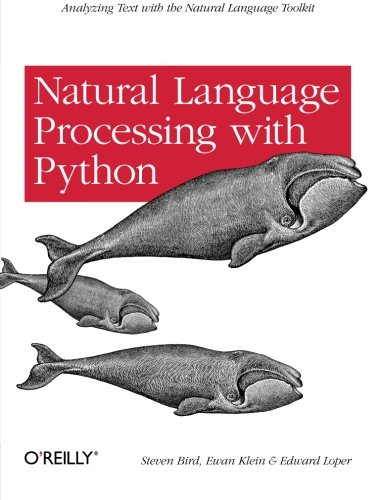
\includegraphics[width=0.15\textwidth]{nltk-buch-python.jpg}
}

\begin{textbox}{Basics of NLTK (Natural Language Toolkit)}
Natural Language versus Artificial Language (i.e. mathematical notations, etc.)

NumPy and Matplotlib have to be installed to generate plots! (should be included in Anaconda anyway)

\begin{quote}
    \lbrack{}Programming/Learning Python-NLTK\rbrack{} is just like learning idiomatic expressions in a foreign language: you're able to buy a nice pastry without first having learned the intricacies of question formation.\footcite[xii]{pythonnltk}
\end{quote}

\end{textbox}


\begin{codebox}{py}{First steps in Python}
# press CTRL+ENTER to evaluate in Jupyter
# mit '#' markiert man Kommentare, also Infos für sich selbst, die der Computer aber ignorieren soll
1 * 4 + 5 / 8
# wie funktionieren die Klammern??

# Grundlegende Funktionalitäten sind bereits in der Standard-Bibliothek enthalten. Für Spezielleres müssen wir sog. 'Pakete' hineinladen. Das geht z.B. so:
import nltk 
nltk.download() # Der Schritt ist nur 1x nötig, wenn das halt noch nicht installiert ist oder out-of-date oder man nicht alles gedownloaded hat beim letzten Mal und jetzt noch andere Sachen dazunehmen will (Paket ist relativ groß, daher könnte es von Interesse sein, nur selektiv manche Sachen zu nehmen)
# nicht vergessen im Prompt/Dialog zu klicken, was man will (Progressbar startet), sonst passiert nix

from nltk.book import *
text1 # Moby Dick
\end{codebox}

\begin{codebox}{py}{\href{https://www.nltk.org/book/ch01.html}{Easy out-of-the-box things to get started}}
import nltk
nltk.download()
from nltk.book import *
text1 # Moby Dick

text1.concordance("monstrous")
text1.similar("monstrous")
text2.similar("monstrous")
text2.common_contexts(["monstrous", "very"])
# import numpy, matplotlib
text4.dispersion_plot(["citizens", "democracy", "freedom", "duties", "America"])
# NumPy and Matplotlib are needed to plot this

len(text3) # word count
sorted(set(text3)) # list unique words in sorted order
len(set(text3)) / len(text3) # number of word types / tokens = measure of lexical diversity
text3.count("smote") # word count for 'smote'
100 * text4.count('a') / len(text4) # percentage of 'a' in text

def lexical_diversity(text): # define this as function
    return len(set(text)) / len(text)
    
def percentage(count, total): # has to define above of the first usage!
    return 100 * count / total

lexical_diversity(text3)
percentage(4, 5)
percentage(text4.count('a'), len(text4))
\end{codebox}

\begin{codebox}{py}{Texts as lists of words}
sent1 = ['Call', 'me', 'Ishmael', '.'] # Moby Dick first sentence as words in list
# stored in a variable named 'sent1' 
# attention: var names are case-sensitive, so sent1 is not the same as Sent1
# some theoretically possible names (like 'not') are reserved words and thus not allowed as variable names. You will be notified by an error.
sent2 # (if you get an error which says that sent2 is not defined, you need to first type  from nltk.book import * ) 
sent4 + sent1 # concatenation (adding strings / text)
sent1.append("Some")
sent1 # word has been appended
text4[173] # get element via numeric index
# the first index always starts with 0, thus the last is (len(thingy) -1) 
text4.index('awaken') # find out this index for a specific word
text5[16715:16735] # getting elements like this is called 'slicing'
\end{codebox}

\begin{codebox}{py}{Texts as lists of words}
name = 'Monty'
name[0] # a word/string can be processed just like a list
name[:4] # get first 4 characters
name + '!'
' '.join(['Monty', 'Python']) # joined together with one whitespace as 'glue'
'Monty Python'.split() # splitted into a list

# How can we automatically identify the words of a text that are most informative about the topic and genre of the text? Get the most frequent 50 (mfw = most frequent words)
fdist1 = FreqDist(text1) # frequency distribution
print(fdist1)
fdist1.most_common(50)
fdist1['whale']

Vocab = set(text1)
# get all the words from the vocabulary which are longer than 15 characters as a list
long_words = [w for w in Vocab if len(w) > 15] 
# w is an arbitrary shorthand for w
# you could also just say 'word' but it's longer to type it
sorted(long_words)
\end{codebox}

\begin{codebox}{py}{Texts as lists of words}
# [NLP book, Chap. 3.2] very long words are often hapaxes (i.e., unique) and perhaps it would be better to find frequently occurring long words. This seems promising since it eliminates frequent short words (e.g., the) and infrequent long words (e.g. antiphilosophists). Here are all words from the chat corpus that are longer than seven characters, that occur more than seven times:
sorted(w for w in set(text5) if len(w) > 7 and fdist1[w] > 7)

# [NLP book, Chap. 3.3] A collocation is a sequence of words that occur together unusually often. Thus red wine is a collocation, whereas the wine is not. A characteristic of collocations is that they are resistant to substitution with words that have similar senses; for example, maroon wine sounds definitely odd. To get a handle on collocations, we start off by extracting from a text a list of word pairs, also known as bigrams.
list(bigrams(['more', 'is', 'said', 'than', 'done']))
text4.collocations()
text8.collocations()

fdist1.tabulate()
fdist1.plot()

sorted(w for w in set(text1) if w.endswith('ableness'))
sorted(term for term in set(text4) if 'gnt' in term)
[w.upper() for w in text1] # capitalize words
len(set(word.lower() for word in text1)) # case-folded list of words
\end{codebox}

\begin{codebox}{py}{Nested conditions}
if len(word) >= 5:
    print('word length is greater than or equal to 5')
for word in ['Call', 'me', 'Ishmael', '.']:
    print(word)

sent1 = ['Call', 'me', 'Ishmael', '.']
for xyzzy in sent1:
    if xyzzy.endswith('l'):
        print(xyzzy)
        print(xyzzy, end=' ') # print not as newline but space-separated
\end{codebox}

\begin{textbox}{Basics of CLTK (Classical Language Toolkit)}
\protect\url{http://cltk.org/} \sep
\href{http://docs.cltk.org/en/latest/installation.html}{CLTK-Installation Page}

\begin{verbatim}
    python3 -m venv venv
    source venv/bin/activate
    pip install cltk
\end{verbatim}
\mycommand{sudo apt-get install python-dev}{If error (missing Python.h)}

\begin{verbatim}
sudo apt update
sudo apt install git
sudo apt-get install python-setuptools
sudo apt install python-virtualenv
virtualenv -p python3 ~/venv
source ~/venv/bin/activate
pip3 install cltk
\end{verbatim}

Install from source: Clone from Github, then:
\begin{verbatim}
    pip install -U -r requirements.txt
    python setup.py install
\end{verbatim}

In the following code boxes are some example usages.
There are many more tutorials on the CLTK Github (accessible through the project web page) such as Lemmatization, Creating a Lexical Disperion Plot, etc.
\end{textbox}

\begin{textbox}{Further CLTK troubleshooting}
\href{https://github.com/cltk/tutorials/blob/master/1%20CLTK%20Setup.ipynb}{Setup Tutorial}

In den Ordner navigieren, wo CLTK ist \sep 
Jupyter Notebook von dort aus  starten, sonst kann es kein CLTK.
\end{textbox}

\begin{codebox}{py}{J-i u-v replacement}
# Converting J to I, V to U
from cltk.stem.latin.j_v import JVReplacer

j = JVReplacer()
j.replace('vem jam') #Out[3]: 'uem iam'
\end{codebox}

\begin{codebox}{py}{Declining using Collatinus}
from cltk.stem.latin.declension import CollatinusDecliner

decliner = CollatinusDecliner()

print(decliner.decline("via"))
decliner.decline("via", flatten=True)
\end{codebox}

\begin{codebox}{py}{Lemmatizer}
# The CLTK offers a series of lemmatizers that can be combined in a backoff chain, i.e. if one lemmatizer is unable to return a headword for a token, this token can be passed onto another lemmatizer until either a headword is returned or the sequence ends.
from cltk.lemmatize.latin.backoff import BackoffLatinLemmatizer

lemmatizer = BackoffLatinLemmatizer()
tokens = ['Quo', 'usque', 'tandem', 'abutere', ',', 'Catilina', ',', 'patientia', 'nostra', '?']
lemmatizer.lemmatize(tokens)
\end{codebox}

\begin{codebox}{py}{Line Tokenization}
from cltk.tokenize.line import LineTokenizer

tokenizer = LineTokenizer('latin')
untokenized_text = """49. Miraris verbis nudis me scribere versus?\nHoc brevitas fecit, sensus coniungere binos."""
tokenizer.tokenize(untokenized_text)
\end{codebox}

\begin{codebox}{py}{Stopword Removal}
from nltk.tokenize.punkt import PunktLanguageVars
from cltk.stop.latin.stops import STOPS_LIST

sentence = 'Quo usque tandem abutere, Catilina, patientia nostra?'
p = PunktLanguageVars()
tokens = p.word_tokenize(sentence.lower())
[w for w in tokens if not w in STOPS_LIST]
# alternative to this Perseus list, a custom stop list can be built, see docs
\end{codebox}

\begin{codebox}{py}{Macronizer}
# Macronizer: Automatically mark long Latin vowels with a macron. 
# Note that the macronizer’s accuracy varies depending on which tagger is used.
# macronized text is needed for scansion (see below)

from cltk.prosody.latin.macronizer import Macronizer
macronizer = Macronizer('tag_ngram_123_backoff')

text = 'Quo usque tandem, O Catilina, abutere nostra patientia?'
macronizer.macronize_text(text)
# Out[4]: 'quō usque tandem , ō catilīnā , abūtēre nostrā patientia ?
macronizer.macronize_tags(text) # alternatively
\end{codebox}

\begin{codebox}{py}{CLTK Scansion}
from cltk.prosody.latin.scanner import Scansion
from cltk.prosody.latin.clausulae_analysis import Clausulae

text = 'quō usque tandem abūtēre, Catilīna, patientiā nostrā. quam diū etiam furor iste tuus nōs ēlūdet.'

s = Scansion()
c = Clausulae()

prosody = s.scan_text(text) #Out[6]: ['-uuu-uuu-u--x', 'uu-uu-uu----x']

c.clausulae_analysis(prosody)
\end{codebox}

\begin{codebox}{py}{Prosody Scanner}
# A prosody scanner is available for text which already has had its natural lengths marked with macrons. It returns a list of strings of long and short marks for each sentence, with an anceps marking the last syllable of each sentence.
# The algorithm is designed only for Latin prose rhythms. It is detailed in Keeline, T. and Kirby, J “Auceps syllabarum: A Digital Analysis of Latin Prose Rhythm,” Journal of Roman Studies, 2019.
from cltk.prosody.latin.scanner import Scansion
scanner = Scansion()
text = 'quō usque tandem abūtēre, Catilīna, patientiā nostrā. quam diū etiam furor iste tuus nōs ēlūdet.'
scanner.scan_text(text)
\end{codebox}

\begin{codebox}{py}{HexameterScanner}
from cltk.prosody.latin.hexameter_scanner import HexameterScanner
scanner = HexameterScanner()
scanner.scan("impulerit. Tantaene animis caelestibus irae?")
\end{codebox}


\begin{codebox}{py}{PentameterScanner}
from cltk.prosody.latin.pentameter_scanner import PentameterScanner
scanner = PentameterScanner()
scanner.scan("ex hoc ingrato gaudia amore tibi.")
# for more see http://docs.cltk.org/en/latest/latin.html
# HendecasyllableScanner, Syllabifier, etc.
\end{codebox}
\begin{codebox}{py}{Named Entity Recognition}
# There is available a simple interface to a list of Latin proper nouns (see repo for how  the list was created). 
# Ergo: will recognize personal names from the list (thus you can add your own!)
from cltk.tag import ner
from cltk.stem.latin.j_v import JVReplacer

text_str = """ut Venus, ut Sirius, ut Spica, ut aliae quae primae dicuntur esse mangitudinis."""
jv_replacer = JVReplacer()
text_str_iu = jv_replacer.replace(text_str)

ner.tag_ner('latin', input_text=text_str_iu, output_type=list)
\end{codebox}


\section{CLTK Pipeline}
\begin{codebox}{py}{Corpus Import}
# available as tutorial Jupyter Notebooks from the CLTK Github
# https://github.com/cltk/tutorials/blob/master/2%20Import%20corpora.ipynb
from cltk.corpus.utils.importer import CorpusImporter
my_latin_downloader = CorpusImporter('latin')
my_latin_downloader.list_corpora # show available corpora

my_latin_downloader.import_corpus('latin_text_latin_library')
my_latin_downloader.import_corpus('latin_models_cltk')

# save text in string variable
# Introduction to Cato's De agricultura
cato_agri_praef = "Est interdum praestare mercaturis rem quaerere, nisi tam periculosum sit, et item foenerari, si tam honestum. Maiores nostri sic habuerunt et ita in legibus posiverunt: furem dupli condemnari, foeneratorem quadrupli. Quanto peiorem civem existimarint foeneratorem quam furem, hinc licet existimare. Et virum bonum quom laudabant, ita laudabant: bonum agricolam bonumque colonum; amplissime laudari existimabatur qui ita laudabatur. Mercatorem autem strenuum studiosumque rei quaerendae existimo, verum, ut supra dixi, periculosum et calamitosum. At ex agricolis et viri fortissimi et milites strenuissimi gignuntur, maximeque pius quaestus stabilissimusque consequitur minimeque invidiosus, minimeque male cogitantes sunt qui in eo studio occupati sunt. Nunc, ut ad rem redeam, quod promisi institutum principium hoc erit."


# See http://docs.cltk.org/en/latest/latin.html#sentence-tokenization
from cltk.tokenize.sentence import TokenizeSentence
tokenizer = TokenizeSentence('latin')
cato_sentence_tokens = tokenizer.tokenize_sentences(cato_agri_praef)
print(len(cato_sentence_tokens)) # 9

for sentence in cato_sentence_tokens:
    print(sentence)
    print()

# Import general-use word tokenizer
from cltk.tokenize.word import nltk_tokenize_words
cato_word_tokens = nltk_tokenize_words(cato_agri_praef)
print(cato_word_tokens)
cato_word_tokens_no_punt = [token for token in cato_word_tokens if token not in ['.', ',', ':', ';']]
# you can remove duplicates by using the set() function on it

# There's a mistake here, though:
# capitalized words ('At', 'Est', 'Nunc') would be counted incorrectly.
# So let's lowercase the input string and try again:

cato_agri_praef_lowered = cato_agri_praef.lower()
cato_word_tokens_lowered = nltk_tokenize_words(cato_agri_praef_lowered)
\end{codebox}

\begin{codebox}{py}{Visualize word frequencies}
from collections import Counter
# You don't get the unique word forms, but count all tokens

cato_word_counts_counter = Counter(cato_cltk_word_tokens_no_punt)
print(cato_word_counts_counter)

# Lexical diversity is a simple measure of unique words divided by total words. This measures how relatively verbose an author is. Such lexical measures are simple but can be illuminating nevertheless. 

# Lexical diversity of our little paragraph
print(len(cato_cltk_word_tokens_no_punt_unique) / len(cato_cltk_word_tokens_no_punt))
# This represents the ratio of unique words to re-reused words
\end{codebox}

\begin{codebox}{py}{Text reuse}
# Load all of Cicero's De divinatione
import os
# from your own machine (!)
div1_fp = os.path.expanduser('~/cltk_data/latin/text/latin_text_latin_library/cicero/divinatione1.txt')
div2_fp = os.path.expanduser('~/cltk_data/latin/text/latin_text_latin_library/cicero/divinatione2.txt')

with open(div1_fp) as fo:
    div1 = fo.read()

with open(div2_fp) as fo:
    div2 = fo.read()

# We will calculate the Levenstein distance
# See http://docs.cltk.org/en/latest/multilingual.html#text-reuse
from cltk.text_reuse.levenshtein import Levenshtein
lev_dist = Levenshtein()
lev_dist.ratio(div1, div2)

from cltk.text_reuse.comparison import long_substring

# Aen 1.1-6
aen = """arma virumque cano, Troiae qui primus ab oris
Italiam, fato profugus, Laviniaque venit
litora, multum ille et terris iactatus et alto
vi superum saevae memorem Iunonis ob iram;
multa quoque et bello passus, dum conderet urbem,               5
inferretque deos Latio, genus unde Latinum,
Albanique patres, atque altae moenia Romae."""

# Servius 1.1
serv = """arma multi varie disserunt cur ab armis Vergilius coeperit, omnes tamen inania sentire manifestum est, cum eum constet aliunde sumpsisse principium, sicut in praemissa eius vita monstratum est. per 'arma' autem bellum significat, et est tropus metonymia. nam arma quibus in bello utimur pro bello posuit, sicut toga qua in pace utimur pro pace ponitur, ut Cicero “cedant arma togae” , id est bellum paci. alii ideo 'arma' hoc loco proprie dicta accipiunt, primo quod fuerint victricia, secundo quod divina, tertio quod prope semper armis virum subiungit, ut “arma virumque ferens” et “arma acri facienda viro” . arma virumque figura usitata est ut non eo ordine respondeamus quo proposuimus; nam prius de erroribus Aeneae dicit, post de bello. hac autem figura etiam in prosa utimur. sic Cicero in Verrinis “nam sine ullo sumptu nostro coriis, tunicis frumentoque suppeditato maximos exercitus nostros vestivit, aluit, armavit” . non nulli autem hyperbaton putant, ut sit sensus talis 'arma virumque cano, genus unde Latinum Albanique patres atque altae moenia Romae', mox illa revoces 'Troiae qui primus ab oris'; sic enim causa operis declaratur, cur cogentibus fatis in Latium venerit. et est poeticum principium professivum 'arma virumque cano', invocativum 'Musa mihi causas memora', narrativum 'urbs antiqua fuit'. et professivum quattuor modis sumpsit: a duce 'arma virumque cano', ab itinere 'Troiae qui primus ab oris', a bello 'multa quoque et bello passus', a generis successu 'genus unde Latinum'. virum quem non dicit, sed circumstantiis ostendit Aeneam."""

print(long_substring(aen, serv))
\end{codebox}

%---------------------------------------------
\AtNextBibliography{\footnotesize}
\printbibliography  
\end{multicols}

\end{document}
